\documentclass[12pt,]{article}
\usepackage{lmodern}
\usepackage{amssymb,amsmath}
\usepackage{ifxetex,ifluatex}
\usepackage{fixltx2e} % provides \textsubscript
\ifnum 0\ifxetex 1\fi\ifluatex 1\fi=0 % if pdftex
  \usepackage[T1]{fontenc}
  \usepackage[utf8]{inputenc}
\else % if luatex or xelatex
  \ifxetex
    \usepackage{mathspec}
  \else
    \usepackage{fontspec}
  \fi
  \defaultfontfeatures{Ligatures=TeX,Scale=MatchLowercase}
    \setmainfont[]{Times New Roman}
\fi
% use upquote if available, for straight quotes in verbatim environments
\IfFileExists{upquote.sty}{\usepackage{upquote}}{}
% use microtype if available
\IfFileExists{microtype.sty}{%
\usepackage{microtype}
\UseMicrotypeSet[protrusion]{basicmath} % disable protrusion for tt fonts
}{}
\usepackage[margin=2.54cm]{geometry}
\usepackage{hyperref}
\hypersetup{unicode=true,
            pdftitle={Factors Influencing Above Ground Biomass of Forest Plots in the Congo},
            pdfauthor={Nikki Egna},
            pdfborder={0 0 0},
            breaklinks=true}
\urlstyle{same}  % don't use monospace font for urls
\usepackage{color}
\usepackage{fancyvrb}
\newcommand{\VerbBar}{|}
\newcommand{\VERB}{\Verb[commandchars=\\\{\}]}
\DefineVerbatimEnvironment{Highlighting}{Verbatim}{commandchars=\\\{\}}
% Add ',fontsize=\small' for more characters per line
\usepackage{framed}
\definecolor{shadecolor}{RGB}{248,248,248}
\newenvironment{Shaded}{\begin{snugshade}}{\end{snugshade}}
\newcommand{\AlertTok}[1]{\textcolor[rgb]{0.94,0.16,0.16}{#1}}
\newcommand{\AnnotationTok}[1]{\textcolor[rgb]{0.56,0.35,0.01}{\textbf{\textit{#1}}}}
\newcommand{\AttributeTok}[1]{\textcolor[rgb]{0.77,0.63,0.00}{#1}}
\newcommand{\BaseNTok}[1]{\textcolor[rgb]{0.00,0.00,0.81}{#1}}
\newcommand{\BuiltInTok}[1]{#1}
\newcommand{\CharTok}[1]{\textcolor[rgb]{0.31,0.60,0.02}{#1}}
\newcommand{\CommentTok}[1]{\textcolor[rgb]{0.56,0.35,0.01}{\textit{#1}}}
\newcommand{\CommentVarTok}[1]{\textcolor[rgb]{0.56,0.35,0.01}{\textbf{\textit{#1}}}}
\newcommand{\ConstantTok}[1]{\textcolor[rgb]{0.00,0.00,0.00}{#1}}
\newcommand{\ControlFlowTok}[1]{\textcolor[rgb]{0.13,0.29,0.53}{\textbf{#1}}}
\newcommand{\DataTypeTok}[1]{\textcolor[rgb]{0.13,0.29,0.53}{#1}}
\newcommand{\DecValTok}[1]{\textcolor[rgb]{0.00,0.00,0.81}{#1}}
\newcommand{\DocumentationTok}[1]{\textcolor[rgb]{0.56,0.35,0.01}{\textbf{\textit{#1}}}}
\newcommand{\ErrorTok}[1]{\textcolor[rgb]{0.64,0.00,0.00}{\textbf{#1}}}
\newcommand{\ExtensionTok}[1]{#1}
\newcommand{\FloatTok}[1]{\textcolor[rgb]{0.00,0.00,0.81}{#1}}
\newcommand{\FunctionTok}[1]{\textcolor[rgb]{0.00,0.00,0.00}{#1}}
\newcommand{\ImportTok}[1]{#1}
\newcommand{\InformationTok}[1]{\textcolor[rgb]{0.56,0.35,0.01}{\textbf{\textit{#1}}}}
\newcommand{\KeywordTok}[1]{\textcolor[rgb]{0.13,0.29,0.53}{\textbf{#1}}}
\newcommand{\NormalTok}[1]{#1}
\newcommand{\OperatorTok}[1]{\textcolor[rgb]{0.81,0.36,0.00}{\textbf{#1}}}
\newcommand{\OtherTok}[1]{\textcolor[rgb]{0.56,0.35,0.01}{#1}}
\newcommand{\PreprocessorTok}[1]{\textcolor[rgb]{0.56,0.35,0.01}{\textit{#1}}}
\newcommand{\RegionMarkerTok}[1]{#1}
\newcommand{\SpecialCharTok}[1]{\textcolor[rgb]{0.00,0.00,0.00}{#1}}
\newcommand{\SpecialStringTok}[1]{\textcolor[rgb]{0.31,0.60,0.02}{#1}}
\newcommand{\StringTok}[1]{\textcolor[rgb]{0.31,0.60,0.02}{#1}}
\newcommand{\VariableTok}[1]{\textcolor[rgb]{0.00,0.00,0.00}{#1}}
\newcommand{\VerbatimStringTok}[1]{\textcolor[rgb]{0.31,0.60,0.02}{#1}}
\newcommand{\WarningTok}[1]{\textcolor[rgb]{0.56,0.35,0.01}{\textbf{\textit{#1}}}}
\usepackage{longtable,booktabs}
\usepackage{graphicx,grffile}
\makeatletter
\def\maxwidth{\ifdim\Gin@nat@width>\linewidth\linewidth\else\Gin@nat@width\fi}
\def\maxheight{\ifdim\Gin@nat@height>\textheight\textheight\else\Gin@nat@height\fi}
\makeatother
% Scale images if necessary, so that they will not overflow the page
% margins by default, and it is still possible to overwrite the defaults
% using explicit options in \includegraphics[width, height, ...]{}
\setkeys{Gin}{width=\maxwidth,height=\maxheight,keepaspectratio}
\IfFileExists{parskip.sty}{%
\usepackage{parskip}
}{% else
\setlength{\parindent}{0pt}
\setlength{\parskip}{6pt plus 2pt minus 1pt}
}
\setlength{\emergencystretch}{3em}  % prevent overfull lines
\providecommand{\tightlist}{%
  \setlength{\itemsep}{0pt}\setlength{\parskip}{0pt}}
\setcounter{secnumdepth}{5}
% Redefines (sub)paragraphs to behave more like sections
\ifx\paragraph\undefined\else
\let\oldparagraph\paragraph
\renewcommand{\paragraph}[1]{\oldparagraph{#1}\mbox{}}
\fi
\ifx\subparagraph\undefined\else
\let\oldsubparagraph\subparagraph
\renewcommand{\subparagraph}[1]{\oldsubparagraph{#1}\mbox{}}
\fi

%%% Use protect on footnotes to avoid problems with footnotes in titles
\let\rmarkdownfootnote\footnote%
\def\footnote{\protect\rmarkdownfootnote}

%%% Change title format to be more compact
\usepackage{titling}

% Create subtitle command for use in maketitle
\providecommand{\subtitle}[1]{
  \posttitle{
    \begin{center}\large#1\end{center}
    }
}

\setlength{\droptitle}{-2em}

  \title{Factors Influencing Above Ground Biomass of Forest Plots in the Congo}
    \pretitle{\vspace{\droptitle}\centering\huge}
  \posttitle{\par}
  \subtitle{\url{https://github.com/nikki-egna/ENV872_Final_Project_Congo_Carbon}}
  \author{Nikki Egna}
    \preauthor{\centering\large\emph}
  \postauthor{\par}
    \date{}
    \predate{}\postdate{}
  

\begin{document}
\maketitle
\begin{abstract}
Add the abstract here
\end{abstract}

\newpage
\tableofcontents 
\newpage
\listoftables 
\newpage
\listoffigures

\newpage

\hypertarget{rationale-and-research-questions}{%
\section{Rationale and Research
Questions}\label{rationale-and-research-questions}}

Above ground biomass can be a predictor of overall health of a forest
ecosystem. It is also important for looking at carbon storage potential
of forests, which has significant implications for climate change
mitigation. (Ducanson et al., 2019) This study aims to look at various
environmental factors, and how they might contribute to differences in
above ground biomass. The environmental factors included in this study
are Human Footprint Index (HFI), GlobCover, annual precipitation, soil
type, distance from the nearest road, distance from the nearest village,
distance from the nearest river, distance from the nearest saw mill, and
distance from the nearest protected area.

\textbf{Question 1:}

How has above ground biomass changed over time at the plot locations?

\textbf{Question 2:}

Which environmental factors are signicant predictors of above ground
biomass?

\newpage

\hypertarget{dataset-information}{%
\section{Dataset Information}\label{dataset-information}}

This repository uses data from the Poulsen Tropical Ecology Lab, and
contains information on tree diameter and species from plots in the
Congo. This data is being collected in order to model the amount of
above ground biomass (AGB) within each plot across the study sites.
Utilizing remote sensing techniques, the Poulsen Lab performed analysis
to determine several covariate values at each plot, including distance
to nearest road, distance to nearest village, distance to nearest river,
distance to nearest protected area, Human Footprint Index, and Globcover
value. This project will look at which covariates have a significant
impact on AGB at the study sites.

The CongoCarbon\_Raw\_Data.csv was collected by the Poulsen Tropical
Ecology Lab, and their on-ground team based in the Congo. This data is
not public facing, and access was granted through Dr.~John Poulsen. The
CongoCarbon\_AGB\_by\_Plot.csv was created by John Poulsen, Anna
Nordseth, and Nikki Egna based on the raw data. The covariate data
(CongoCarbon\_Plot\_Covariates.csv) was created by Nikki Egna in March
of 2020, and the data it utilizes was obtained from the following
sources: Human Footprint Index was derived from Wildlife Conservation
Society (WCS), Center for International Earth Science Information
Network (CIESIN), and Columbia University and was accessed in December
of 2019. The GlobCover raster was downloaded from the ESA Globcover 2005
Project, led by MEDIAS-France/POSTEL, in December of 2019. Precipitation
data was obtained from the Climate Hazards group Infrared Precipitation
with Stations (CHIRPS) in December of 2019. The roads, river, soil, saw
mill, and villages data comes from the Ministère de l'Économie
Forestière CNIAF\_MEFDD (\url{https://cog.forest-atlas.org}), accessed
in April, 2020.

\hypertarget{metadata}{%
\subsection{Metadata}\label{metadata}}

\hypertarget{congocarbon_raw_data.csv}{%
\subsubsection{CongoCarbon\_Raw\_data.csv}\label{congocarbon_raw_data.csv}}

\begin{longtable}[]{@{}ll@{}}
\toprule
Column Name & Description\tabularnewline
\midrule
\endhead
Tree ID & Identification number assigned to the unique tree
(Numeric)\tabularnewline
Tag No & Secondary tree identification number (Numeric)\tabularnewline
Plot & Study plot number (Numeric)\tabularnewline
Subplot & Subplot number within each plot (Numeric)\tabularnewline
Family & Tree family name (Character)\tabularnewline
Species & Tree species name (Character)\tabularnewline
WD & Wood density (Numeric)\tabularnewline
DBH0\_05 & First diameter measurement in 2005 (Numeric;
Centimeters)\tabularnewline
DBH1\_05 & Second diameter measurement in 2005 (Numeric;
Centimeters)\tabularnewline
DBH2\_05 & Third diameter measurement in 2005 (Numeric;
Centimeters)\tabularnewline
DBH3\_05 & Fourth diameter measurement in 2005 (Numeric;
Centimeters)\tabularnewline
DBH4\_05 & Fifth diameter measurement in 2005 (Numeric;
Centimeters)\tabularnewline
DBH0\_09 & First diameter measurement in 2009 (Numeric;
Centimeters)\tabularnewline
DBH1\_09 & Second diameter measurement in 2009 (Numeric;
Centimeters)\tabularnewline
DBH2\_09 & Third diameter measurement in 2009 (Numeric;
Centimeters)\tabularnewline
DBH3\_09 & Fourth diameter measurement in 2009 (Numeric;
Centimeters)\tabularnewline
DBH4\_09 & Fifth diameter measurement in 2009 (Numeric;
Centimeters)\tabularnewline
DBH0\_13 & First diameter measurement in 2013 (Numeric;
Centimeters)\tabularnewline
DBH1\_13 & Second diameter measurement in 2013 (Numeric;
Centimeters)\tabularnewline
DBH2\_13 & Third diameter measurement in 2013 (Numeric;
Centimeters)\tabularnewline
DBH3\_13 & Fourth diameter measurement in 2013 (Numeric;
Centimeters)\tabularnewline
DBH4\_13 & Fifth diameter measurement in 2013 (Numeric;
Centimeters)\tabularnewline
AGB05.MgE & AGB estimate 2005 (Numeric; milligrams)\tabularnewline
AGB09.MgE & AGB estimate 2009 (Numeric; milligrams)\tabularnewline
AGB13.MgE & AGB estimate 2013 (Numeric; milligrams)\tabularnewline
\bottomrule
\end{longtable}

\hypertarget{congocarbon_plot_covariates.csv}{%
\subsubsection{CongoCarbon\_Plot\_Covariates.csv}\label{congocarbon_plot_covariates.csv}}

\begin{longtable}[]{@{}ll@{}}
\toprule
\begin{minipage}[b]{0.53\columnwidth}\raggedright
Column Name\strut
\end{minipage} & \begin{minipage}[b]{0.41\columnwidth}\raggedright
Description\strut
\end{minipage}\tabularnewline
\midrule
\endhead
\begin{minipage}[t]{0.53\columnwidth}\raggedright
Plot\strut
\end{minipage} & \begin{minipage}[t]{0.41\columnwidth}\raggedright
Tree plot ID number (Factor)\strut
\end{minipage}\tabularnewline
\begin{minipage}[t]{0.53\columnwidth}\raggedright
Latitude\strut
\end{minipage} & \begin{minipage}[t]{0.41\columnwidth}\raggedright
Latitude of the plot (Numeric)\strut
\end{minipage}\tabularnewline
\begin{minipage}[t]{0.53\columnwidth}\raggedright
Longitude\strut
\end{minipage} & \begin{minipage}[t]{0.41\columnwidth}\raggedright
Longitude of the plot (Numeric)\strut
\end{minipage}\tabularnewline
\begin{minipage}[t]{0.53\columnwidth}\raggedright
HFI\strut
\end{minipage} & \begin{minipage}[t]{0.41\columnwidth}\raggedright
Human Footprint Index value at the plot location (Factor)\strut
\end{minipage}\tabularnewline
\begin{minipage}[t]{0.53\columnwidth}\raggedright
GlobCover\strut
\end{minipage} & \begin{minipage}[t]{0.41\columnwidth}\raggedright
GlobCover vegetation index value at the plot location (Factor)\strut
\end{minipage}\tabularnewline
\begin{minipage}[t]{0.53\columnwidth}\raggedright
Precip\_sum\_2013\strut
\end{minipage} & \begin{minipage}[t]{0.41\columnwidth}\raggedright
Annual precipitation sum for 2013 at plot location (Numeric;
millimeters)\strut
\end{minipage}\tabularnewline
\begin{minipage}[t]{0.53\columnwidth}\raggedright
Soil\strut
\end{minipage} & \begin{minipage}[t]{0.41\columnwidth}\raggedright
Soil type index at plot location (Factor)\strut
\end{minipage}\tabularnewline
\begin{minipage}[t]{0.53\columnwidth}\raggedright
Dist\_Road\_m\strut
\end{minipage} & \begin{minipage}[t]{0.41\columnwidth}\raggedright
Distance from plot to the nearest road (Numeric; Meters)\strut
\end{minipage}\tabularnewline
\begin{minipage}[t]{0.53\columnwidth}\raggedright
Dist\_Village\_m\strut
\end{minipage} & \begin{minipage}[t]{0.41\columnwidth}\raggedright
Distance from plot to the nearest village (Numeric; Meters)\strut
\end{minipage}\tabularnewline
\begin{minipage}[t]{0.53\columnwidth}\raggedright
Dist\_River\_m\strut
\end{minipage} & \begin{minipage}[t]{0.41\columnwidth}\raggedright
Distance from plot to the nearest river (Numeric; Meters)\strut
\end{minipage}\tabularnewline
\begin{minipage}[t]{0.53\columnwidth}\raggedright
Dist\_PA\_m\strut
\end{minipage} & \begin{minipage}[t]{0.41\columnwidth}\raggedright
Distance from plot to the nearest protected area (Numeric; Meters)\strut
\end{minipage}\tabularnewline
\begin{minipage}[t]{0.53\columnwidth}\raggedright
Dist\_Saw\_Mills\_m\strut
\end{minipage} & \begin{minipage}[t]{0.41\columnwidth}\raggedright
Distance from plot to the nearest saw mill (Numeric; Meters)\strut
\end{minipage}\tabularnewline
\bottomrule
\end{longtable}

\newpage

\hypertarget{exploratory-analysis}{%
\section{Exploratory Analysis}\label{exploratory-analysis}}

\hypertarget{raw-data}{%
\subsection{Raw Data}\label{raw-data}}

\begin{Shaded}
\begin{Highlighting}[]
\CommentTok{#Check first few rows of data and the structure of the data}
\KeywordTok{head}\NormalTok{(Raw_CongoCarbon_Data)}
\KeywordTok{str}\NormalTok{(Raw_CongoCarbon_Data)}

\CommentTok{#Check class of necessary columns}
\KeywordTok{lapply}\NormalTok{(Raw_CongoCarbon_Data, class)}

\CommentTok{#Change necessary classes}
\NormalTok{Raw_CongoCarbon_Data}\OperatorTok{$}\NormalTok{Plot <-}\StringTok{ }\KeywordTok{as.factor}\NormalTok{(Raw_CongoCarbon_Data}\OperatorTok{$}\NormalTok{Plot)}

\CommentTok{#Check for NAs}
\KeywordTok{anyNA}\NormalTok{(Raw_CongoCarbon_Data}\OperatorTok{$}\NormalTok{AGB05.MgE)}
\KeywordTok{anyNA}\NormalTok{(Raw_CongoCarbon_Data}\OperatorTok{$}\NormalTok{AGB09.MgE)}
\KeywordTok{anyNA}\NormalTok{(Raw_CongoCarbon_Data}\OperatorTok{$}\NormalTok{AGB13.MgE)}

\CommentTok{#Look at number of NA values}
\KeywordTok{nrow}\NormalTok{(}\KeywordTok{subset}\NormalTok{(Raw_CongoCarbon_Data, }\KeywordTok{is.na}\NormalTok{(AGB05.MgE)))}
\KeywordTok{nrow}\NormalTok{(}\KeywordTok{subset}\NormalTok{(Raw_CongoCarbon_Data, }\KeywordTok{is.na}\NormalTok{(AGB09.MgE)))}
\KeywordTok{nrow}\NormalTok{(}\KeywordTok{subset}\NormalTok{(Raw_CongoCarbon_Data, }\KeywordTok{is.na}\NormalTok{(AGB13.MgE)))}
\end{Highlighting}
\end{Shaded}

\hypertarget{covariate-data}{%
\subsection{Covariate Data}\label{covariate-data}}

\begin{Shaded}
\begin{Highlighting}[]
\KeywordTok{head}\NormalTok{(CongoCarbon_Covariates)}
\KeywordTok{str}\NormalTok{(CongoCarbon_Covariates)}

\CommentTok{#Check the class for all columns in CongoCarbon_Covariates}
\KeywordTok{lapply}\NormalTok{(CongoCarbon_Covariates, class)}
\end{Highlighting}
\end{Shaded}

\newpage

\hypertarget{analysis}{%
\section{Analysis}\label{analysis}}

\textbf{Wrangle raw datasets to create a final dataframe with covariate
values, sum of AGB for each year, and the change in AGB by year for each
plot location}

\begin{Shaded}
\begin{Highlighting}[]
\CommentTok{#Create columns with the sum AGB by plot for each year '05, '09, '13}
\NormalTok{AGB_by_Plot <-}\StringTok{ }\NormalTok{Raw_CongoCarbon_Data }\OperatorTok
\StringTok{  }\KeywordTok{group_by}\NormalTok{(Plot) }\OperatorTok
\StringTok{  }\KeywordTok{summarize}\NormalTok{(}\DataTypeTok{sum_AGB05 =} \KeywordTok{sum}\NormalTok{(AGB05.MgE, }\DataTypeTok{na.rm =} \OtherTok{TRUE}\NormalTok{), }
            \DataTypeTok{sum_AGB09 =} \KeywordTok{sum}\NormalTok{(AGB09.MgE, }\DataTypeTok{na.rm =} \OtherTok{TRUE}\NormalTok{), }
            \DataTypeTok{sum_AGB13 =} \KeywordTok{sum}\NormalTok{(AGB13.MgE, }\DataTypeTok{na.rm =} \OtherTok{TRUE}\NormalTok{))}

\CommentTok{#Create columns for change in AGB from '05-'09, '09-'13, & '05-'13}
\NormalTok{AGB_by_Plot}\OperatorTok{$}\NormalTok{change0509 <-}\StringTok{ }\KeywordTok{with}\NormalTok{(AGB_by_Plot, sum_AGB09 }\OperatorTok{-}\StringTok{ }\NormalTok{sum_AGB05)}
\NormalTok{AGB_by_Plot}\OperatorTok{$}\NormalTok{change0913 <-}\StringTok{ }\KeywordTok{with}\NormalTok{(AGB_by_Plot, sum_AGB13 }\OperatorTok{-}\StringTok{ }\NormalTok{sum_AGB09)}
\NormalTok{AGB_by_Plot}\OperatorTok{$}\NormalTok{change0513 <-}\StringTok{ }\KeywordTok{with}\NormalTok{(AGB_by_Plot, sum_AGB13 }\OperatorTok{-}\StringTok{ }\NormalTok{sum_AGB05)}

\CommentTok{#Combine AGB_by_Plot and CongoCarbon_Covariates by plot}
\NormalTok{AGB_and_Covariates_by_Plot <-}\StringTok{ }
\StringTok{  }\KeywordTok{merge}\NormalTok{(CongoCarbon_Covariates, AGB_by_Plot, }\DataTypeTok{by=}\StringTok{"Plot"}\NormalTok{)}
\end{Highlighting}
\end{Shaded}

\emph{Prepare data in correct format for analysis and graphing}

\begin{Shaded}
\begin{Highlighting}[]
\CommentTok{#Change dataframe from horizontal to vertical}
\NormalTok{melted_AGB_by_Plot <-}\StringTok{ }\KeywordTok{melt}\NormalTok{(AGB_by_Plot, }\DataTypeTok{id=}\KeywordTok{c}\NormalTok{(}\StringTok{"Plot"}\NormalTok{))}
\CommentTok{#Create a column for year}
\NormalTok{melted_AGB_by_Plot}\OperatorTok{$}\NormalTok{Year <-}\StringTok{ }\NormalTok{melted_AGB_by_Plot}\OperatorTok{$}\NormalTok{variable}
\NormalTok{melted_AGB_by_Plot}\OperatorTok{$}\NormalTok{Year <-}\StringTok{ }\KeywordTok{gsub}\NormalTok{(}\StringTok{"sum_AGB05"}\NormalTok{,}\StringTok{"2005"}\NormalTok{, }
\NormalTok{                                melted_AGB_by_Plot}\OperatorTok{$}\NormalTok{Year, }\DataTypeTok{fixed=}\NormalTok{T)}
\NormalTok{melted_AGB_by_Plot}\OperatorTok{$}\NormalTok{Year <-}\StringTok{ }\KeywordTok{gsub}\NormalTok{(}\StringTok{"sum_AGB09"}\NormalTok{,}\StringTok{"2009"}\NormalTok{, }
\NormalTok{                                melted_AGB_by_Plot}\OperatorTok{$}\NormalTok{Year, }\DataTypeTok{fixed=}\NormalTok{T)}
\NormalTok{melted_AGB_by_Plot}\OperatorTok{$}\NormalTok{Year <-}\StringTok{ }\KeywordTok{gsub}\NormalTok{(}\StringTok{"sum_AGB13"}\NormalTok{,}\StringTok{"2013"}\NormalTok{, }
\NormalTok{                                melted_AGB_by_Plot}\OperatorTok{$}\NormalTok{Year, }\DataTypeTok{fixed=}\NormalTok{T)}

\CommentTok{#Create dataframe for the sum of AGB by plot}
\NormalTok{sum_AGB_by_plot <-}\StringTok{ }\NormalTok{melted_AGB_by_Plot[melted_AGB_by_Plot}\OperatorTok{$}\NormalTok{variable }
                                      \OperatorTok\StringTok{ "sum"}\NormalTok{, ]}
\CommentTok{#Create dataframe for the change in AGB by plot}
\NormalTok{change_AGB_by_plot <-}\StringTok{ }\NormalTok{melted_AGB_by_Plot[melted_AGB_by_Plot}\OperatorTok{$}\NormalTok{variable }
                                         \OperatorTok\StringTok{ "change"}\NormalTok{, ]}
\CommentTok{#Create dataframe for the change in AGB by year}
\NormalTok{AGB_change_by_year <-}\StringTok{ }\NormalTok{change_AGB_by_plot }\OperatorTok
\StringTok{  }\KeywordTok{group_by}\NormalTok{(variable) }\OperatorTok
\StringTok{  }\KeywordTok{summarise}\NormalTok{(}\DataTypeTok{sum=}\KeywordTok{sum}\NormalTok{(value))}

\CommentTok{#Raw data}
\CommentTok{#Add column for percent change}
\NormalTok{Raw_CongoCarbon_Data}\OperatorTok{$}\NormalTok{Percent_Change_}\DecValTok{0513}\NormalTok{ <-}
\StringTok{  }\NormalTok{((Raw_CongoCarbon_Data}\OperatorTok{$}\NormalTok{AGB13}\OperatorTok{-}\NormalTok{Raw_CongoCarbon_Data}\OperatorTok{$}\NormalTok{AGB05)}\OperatorTok{/}
\StringTok{     }\NormalTok{Raw_CongoCarbon_Data}\OperatorTok{$}\NormalTok{AGB05.MgE)}\OperatorTok{*}\DecValTok{100}

\CommentTok{#Subset necessary data}
\NormalTok{Raw_data_subset <-}\StringTok{ }\NormalTok{Raw_CongoCarbon_Data }\OperatorTok
\StringTok{  }\NormalTok{dplyr}\OperatorTok{::}\KeywordTok{select}\NormalTok{(Tree.ID, Plot, AGB05.MgE, AGB09.MgE, AGB13.MgE)}

\CommentTok{#Melt data}
\NormalTok{melted_raw_data <-}\StringTok{ }\KeywordTok{melt}\NormalTok{(Raw_data_subset, }\DataTypeTok{id=}\KeywordTok{c}\NormalTok{(}\StringTok{"Tree.ID"}\NormalTok{,}\StringTok{"Plot"}\NormalTok{))}

\CommentTok{#Create a column for year}
\NormalTok{melted_raw_data}\OperatorTok{$}\NormalTok{Year <-}\StringTok{ }\NormalTok{melted_raw_data}\OperatorTok{$}\NormalTok{variable}
\NormalTok{melted_raw_data}\OperatorTok{$}\NormalTok{Year <-}\StringTok{ }\KeywordTok{gsub}\NormalTok{(}\StringTok{"AGB05.MgE"}\NormalTok{,}\StringTok{"2005"}\NormalTok{, }
\NormalTok{                             melted_raw_data}\OperatorTok{$}\NormalTok{Year, }\DataTypeTok{fixed=}\NormalTok{T)}
\NormalTok{melted_raw_data}\OperatorTok{$}\NormalTok{Year <-}\StringTok{ }\KeywordTok{gsub}\NormalTok{(}\StringTok{"AGB09.MgE"}\NormalTok{,}\StringTok{"2009"}\NormalTok{, }
\NormalTok{                             melted_raw_data}\OperatorTok{$}\NormalTok{Year, }\DataTypeTok{fixed=}\NormalTok{T)}
\NormalTok{melted_raw_data}\OperatorTok{$}\NormalTok{Year <-}\StringTok{ }\KeywordTok{gsub}\NormalTok{(}\StringTok{"AGB13.MgE"}\NormalTok{,}\StringTok{"2013"}\NormalTok{, }
\NormalTok{                             melted_raw_data}\OperatorTok{$}\NormalTok{Year, }\DataTypeTok{fixed=}\NormalTok{T)}
\end{Highlighting}
\end{Shaded}

\hypertarget{data-visualization}{%
\subsection{Data visualization}\label{data-visualization}}

\begin{figure}
\centering
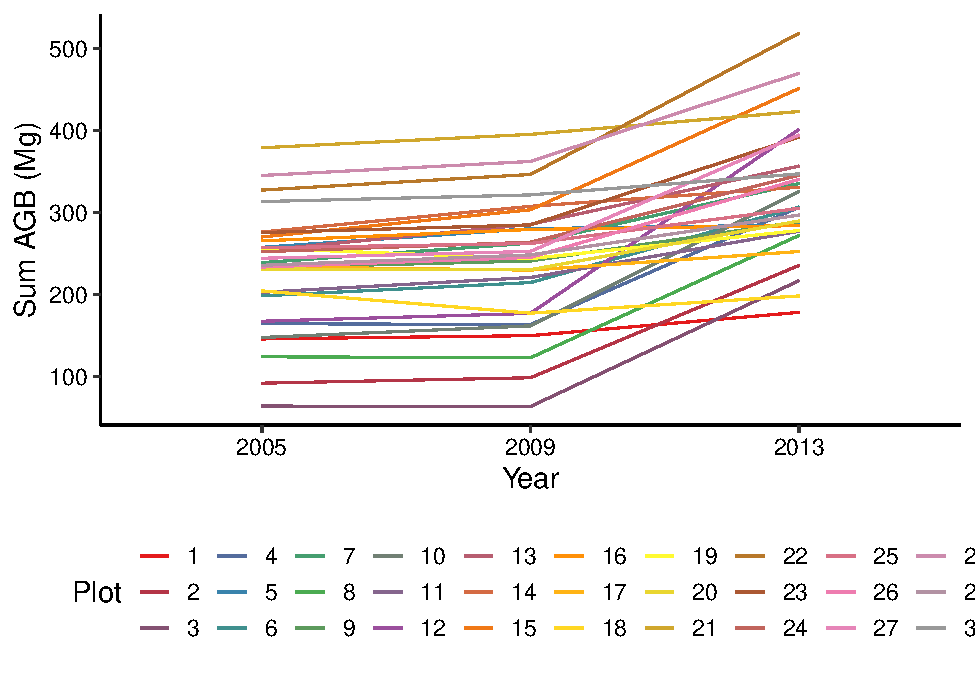
\includegraphics{Project_Template_files/figure-latex/data_visualization-1.pdf}
\caption{Relationship of the changes in total above ground biomass at
each plot between 2005, 2009, and 2013.}
\end{figure}

\begin{figure}
\centering
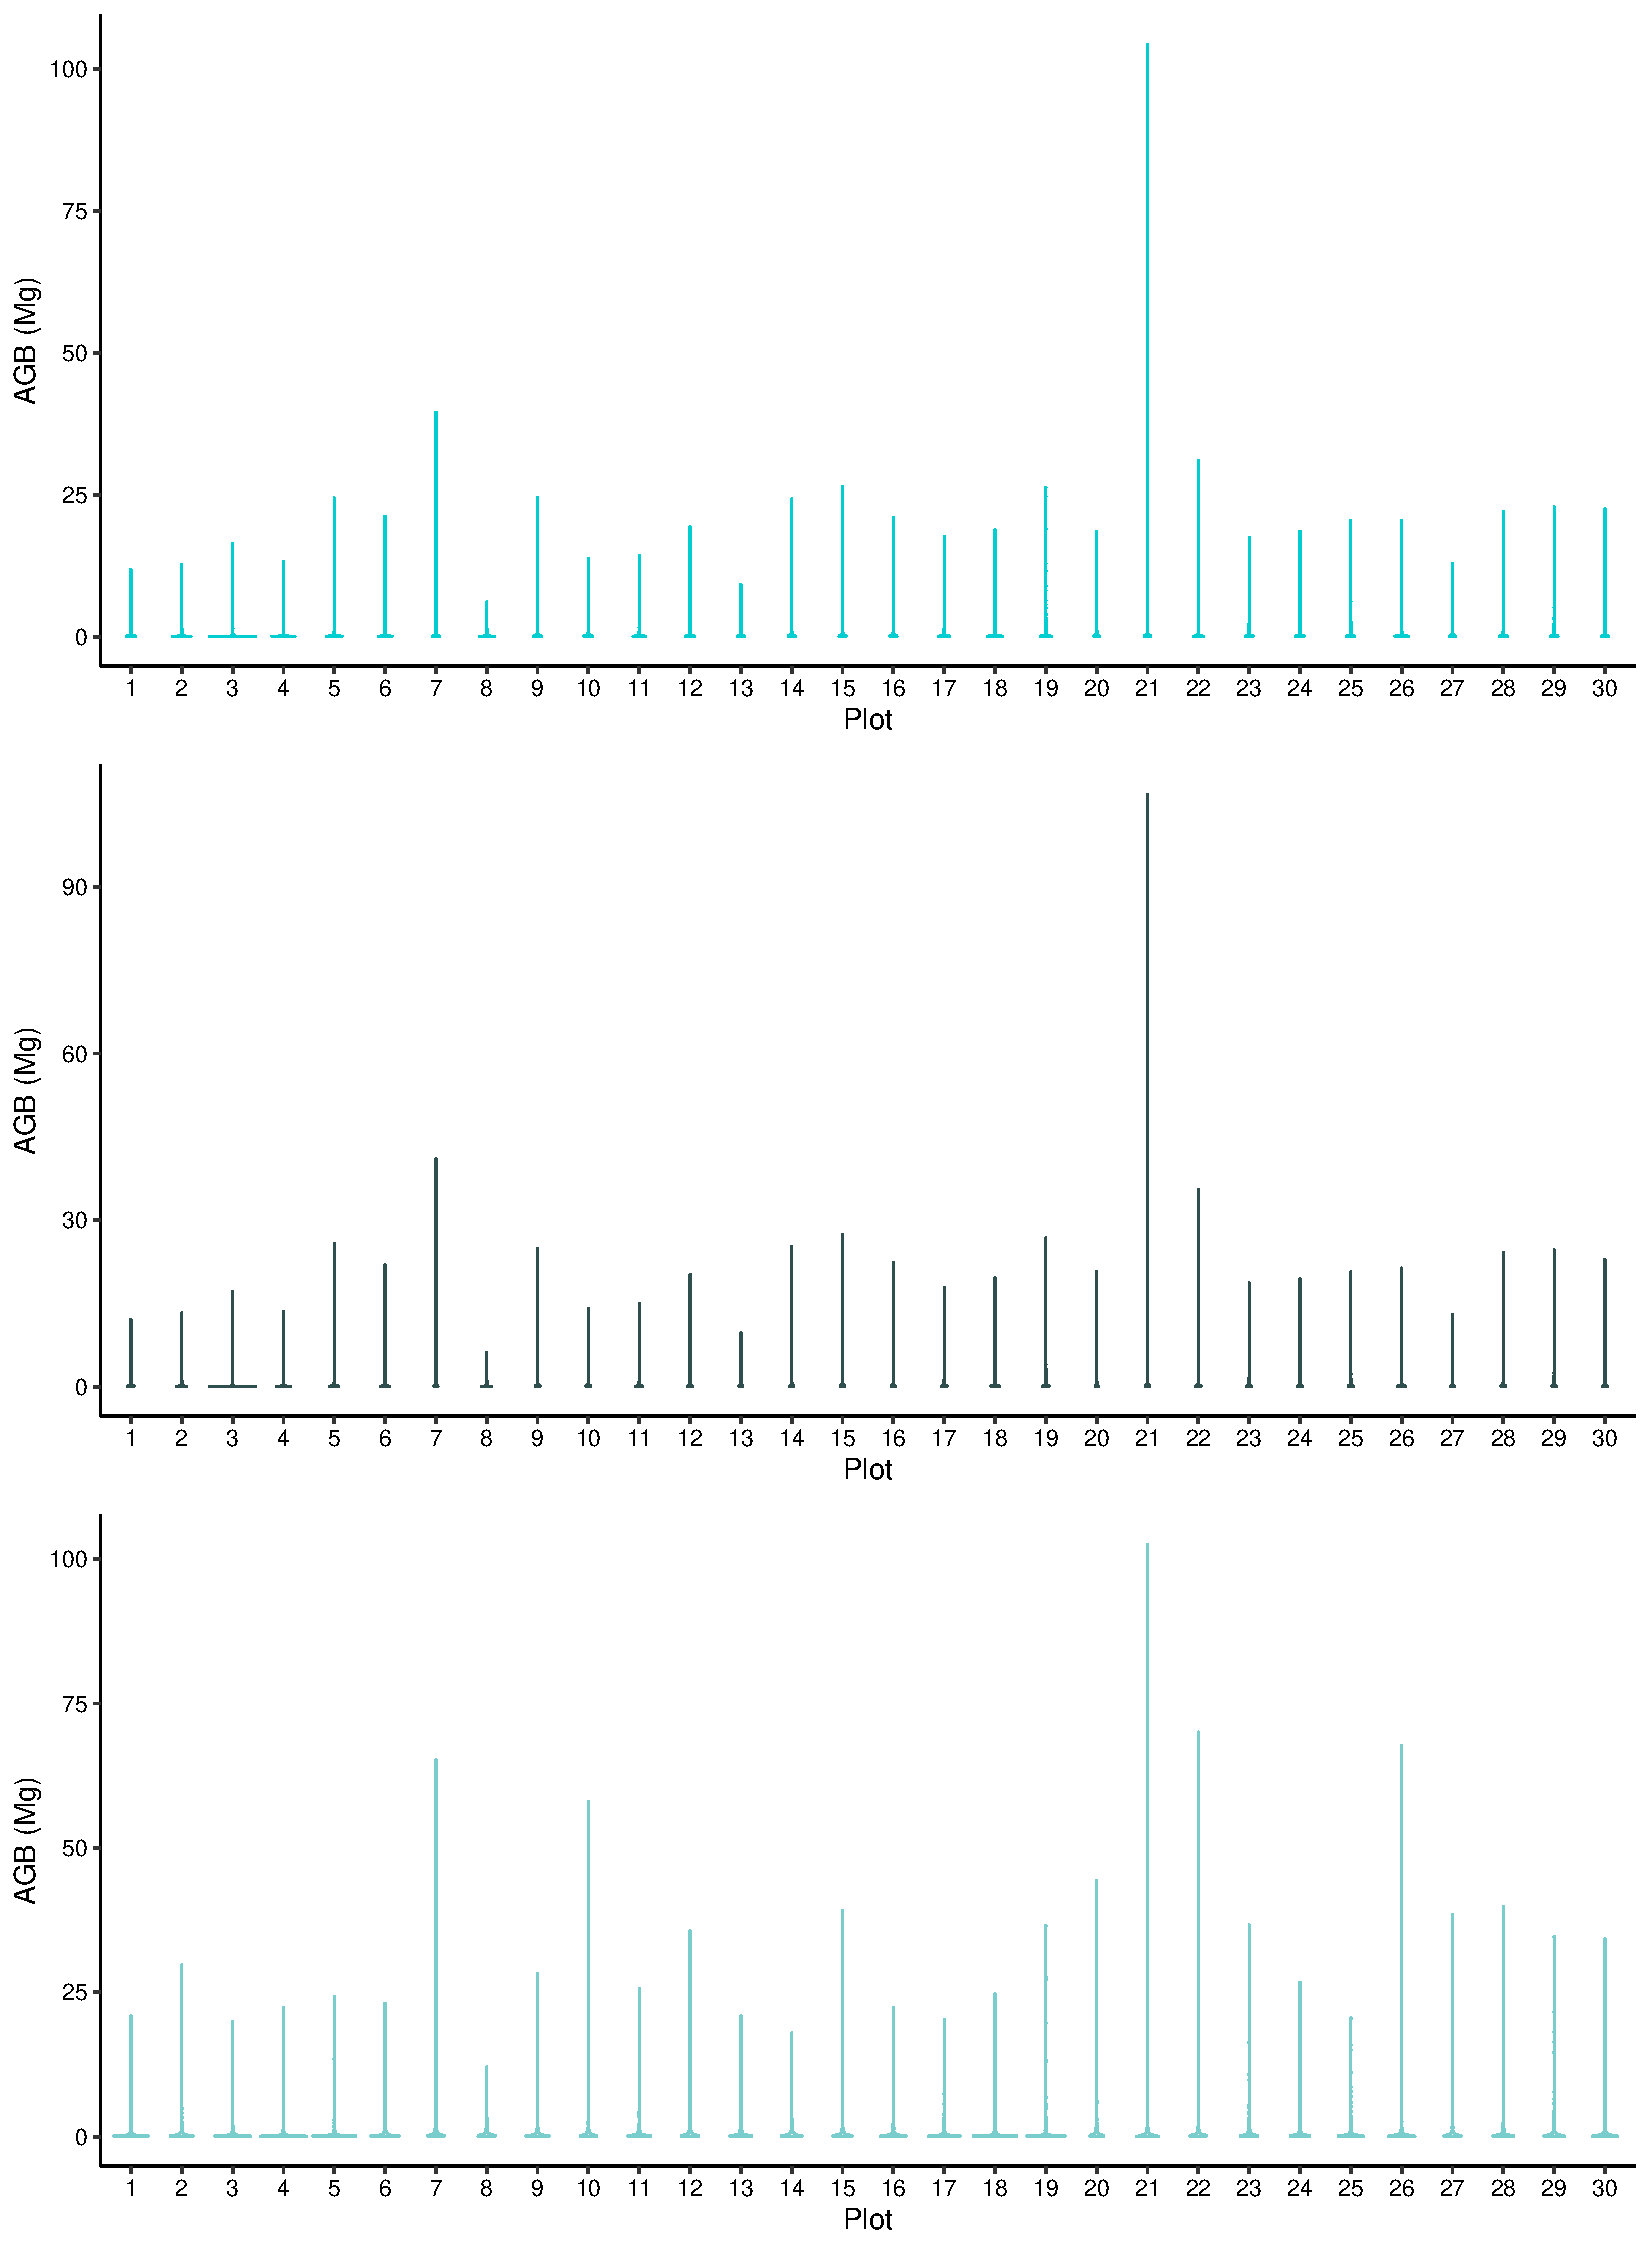
\includegraphics{Project_Template_files/figure-latex/dataviz_2013-1.pdf}
\caption{Relationship between above ground biomass at each plot in
2013.}
\end{figure}

\begin{figure}
\centering
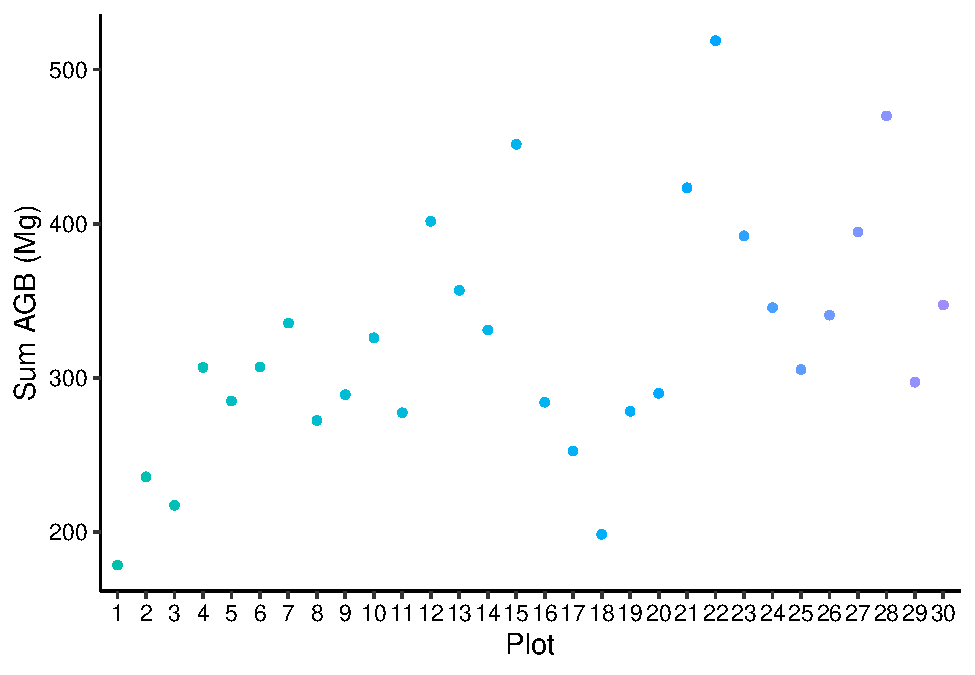
\includegraphics{Project_Template_files/figure-latex/dataviz_sum_2013-1.pdf}
\caption{Relationship between total above ground biomass at each plot in
2013.}
\end{figure}

\hypertarget{question-1-is-there-significant-difference-in-agb-between-each-of-the-years-of-data-collection-2005-2009-and-2013}{%
\subsection{Question 1: Is there significant difference in AGB between
each of the years of data collection (2005, 2009, and
2013)?}\label{question-1-is-there-significant-difference-in-agb-between-each-of-the-years-of-data-collection-2005-2009-and-2013}}

\begin{Shaded}
\begin{Highlighting}[]
\NormalTok{AGB.by.year.model <-}\StringTok{ }\KeywordTok{lm}\NormalTok{(}\DataTypeTok{data=}\NormalTok{melted_raw_data, value }\OperatorTok{~}\StringTok{ }\KeywordTok{as.factor}\NormalTok{(Year))}
\KeywordTok{summary}\NormalTok{(AGB.by.year.model)}
\end{Highlighting}
\end{Shaded}

\begin{verbatim}
## 
## Call:
## lm(formula = value ~ as.factor(Year), data = melted_raw_data)
## 
## Residuals:
##    Min     1Q Median     3Q    Max 
##  -0.91  -0.64  -0.56  -0.30 106.06 
## 
## Coefficients:
##                     Estimate Std. Error t value Pr(>|t|)    
## (Intercept)           0.6136     0.0237   25.94   <2e-16 ***
## as.factor(Year)2009   0.0509     0.0338    1.51     0.13    
## as.factor(Year)2013   0.2939     0.0339    8.68   <2e-16 ***
## ---
## Signif. codes:  0 '***' 0.001 '**' 0.01 '*' 0.05 '.' 0.1 ' ' 1
## 
## Residual standard error: 2.51 on 32750 degrees of freedom
##   (4930 observations deleted due to missingness)
## Multiple R-squared:  0.0026, Adjusted R-squared:  0.00253 
## F-statistic: 42.6 on 2 and 32750 DF,  p-value: <2e-16
\end{verbatim}

\begin{Shaded}
\begin{Highlighting}[]
\KeywordTok{TukeyHSD}\NormalTok{(}\KeywordTok{aov}\NormalTok{(}\DataTypeTok{data=}\NormalTok{melted_raw_data, value }\OperatorTok{~}\StringTok{ }\KeywordTok{as.factor}\NormalTok{(Year)))}
\end{Highlighting}
\end{Shaded}

\begin{verbatim}
##   Tukey multiple comparisons of means
##     95% family-wise confidence level
## 
## Fit: aov(formula = value ~ as.factor(Year), data = melted_raw_data)
## 
## $`as.factor(Year)`
##             diff     lwr   upr p adj
## 2009-2005 0.0509 -0.0282 0.130 0.287
## 2013-2005 0.2939  0.2146 0.373 0.000
## 2013-2009 0.2430  0.1629 0.323 0.000
\end{verbatim}

\hypertarget{question-2-which-environmental-factors-are-significant-predictors-of-agb}{%
\subsection{Question 2: Which environmental factors are significant
predictors of
AGB?}\label{question-2-which-environmental-factors-are-significant-predictors-of-agb}}

\begin{Shaded}
\begin{Highlighting}[]
\CommentTok{#Main effects sum '13}
\NormalTok{AGB.main}\FloatTok{.13}\NormalTok{ <-}\StringTok{ }\KeywordTok{lm}\NormalTok{(}\DataTypeTok{data =}\NormalTok{ AGB_and_Covariates_by_Plot, sum_AGB13 }\OperatorTok{~}\StringTok{ }
\StringTok{                    }\KeywordTok{as.factor}\NormalTok{(HFI) }\OperatorTok{+}\StringTok{ }\KeywordTok{as.factor}\NormalTok{(GlobCover) }\OperatorTok{+}\StringTok{ }\KeywordTok{as.factor}\NormalTok{(Soil) }\OperatorTok{+}
\StringTok{                    }\NormalTok{Precip_sum_}\DecValTok{2013} \OperatorTok{+}\StringTok{ }\NormalTok{Dist_Road_m }\OperatorTok{+}\StringTok{ }\NormalTok{Dist_Village_m }\OperatorTok{+}\StringTok{ }\NormalTok{Dist_PA_m }\OperatorTok{+}\StringTok{ }
\StringTok{                    }\NormalTok{Dist_Saw_Mills_m)}
\CommentTok{#summary(AGB.main.13)}

\CommentTok{#step(AGB.main.13)}

\CommentTok{#Best model}
\NormalTok{AGB.main}\FloatTok{.13}\NormalTok{ <-}\StringTok{ }\KeywordTok{lm}\NormalTok{(}\DataTypeTok{formula =}\NormalTok{ sum_AGB13 }\OperatorTok{~}\StringTok{ }\NormalTok{Precip_sum_}\DecValTok{2013} \OperatorTok{+}\StringTok{ }
\StringTok{                    }\NormalTok{Dist_Road_m }\OperatorTok{+}\StringTok{ }\NormalTok{Dist_Village_m }\OperatorTok{+}\StringTok{ }\NormalTok{Dist_PA_m }\OperatorTok{+}\StringTok{ }
\StringTok{                    }\NormalTok{Dist_Saw_Mills_m, }\DataTypeTok{data =}\NormalTok{ AGB_and_Covariates_by_Plot)}
\NormalTok{AGB.main}\FloatTok{.13}
\end{Highlighting}
\end{Shaded}

\begin{verbatim}
## 
## Call:
## lm(formula = sum_AGB13 ~ Precip_sum_2013 + Dist_Road_m + Dist_Village_m + 
##     Dist_PA_m + Dist_Saw_Mills_m, data = AGB_and_Covariates_by_Plot)
## 
## Coefficients:
##      (Intercept)   Precip_sum_2013       Dist_Road_m    Dist_Village_m  
##        -2.20e+02          3.84e+00          9.83e-03          5.78e-03  
##        Dist_PA_m  Dist_Saw_Mills_m  
##        -7.54e-03         -1.03e-02
\end{verbatim}

\begin{Shaded}
\begin{Highlighting}[]
\KeywordTok{summary}\NormalTok{(AGB.main}\FloatTok{.13}\NormalTok{)}
\end{Highlighting}
\end{Shaded}

\begin{verbatim}
## 
## Call:
## lm(formula = sum_AGB13 ~ Precip_sum_2013 + Dist_Road_m + Dist_Village_m + 
##     Dist_PA_m + Dist_Saw_Mills_m, data = AGB_and_Covariates_by_Plot)
## 
## Residuals:
##    Min     1Q Median     3Q    Max 
##  -98.5  -37.8   -8.5   16.1  181.3 
## 
## Coefficients:
##                   Estimate Std. Error t value Pr(>|t|)  
## (Intercept)      -2.20e+02   4.13e+02   -0.53    0.599  
## Precip_sum_2013   3.84e+00   2.23e+00    1.72    0.099 .
## Dist_Road_m       9.83e-03   5.96e-03    1.65    0.112  
## Dist_Village_m    5.78e-03   3.33e-03    1.73    0.096 .
## Dist_PA_m        -7.54e-03   3.71e-03   -2.03    0.053 .
## Dist_Saw_Mills_m -1.03e-02   5.26e-03   -1.95    0.062 .
## ---
## Signif. codes:  0 '***' 0.001 '**' 0.01 '*' 0.05 '.' 0.1 ' ' 1
## 
## Residual standard error: 65.4 on 24 degrees of freedom
## Multiple R-squared:  0.427,  Adjusted R-squared:  0.307 
## F-statistic: 3.57 on 5 and 24 DF,  p-value: 0.0148
\end{verbatim}

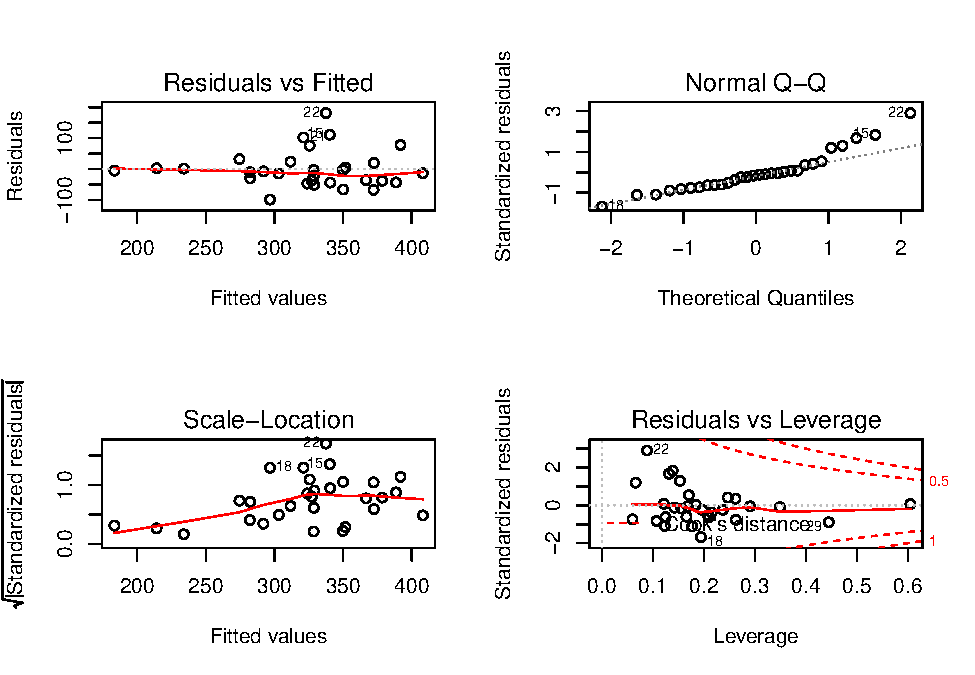
\includegraphics{Project_Template_files/figure-latex/modelfit-1.pdf}
\newpage

\begin{verbatim}
##        Plot    Latitude   Longitude 
## "character"   "numeric"   "numeric"
\end{verbatim}

\begin{verbatim}
## Source : https://maps.googleapis.com/maps/api/staticmap?center=2.195,16.28&zoom=11&size=640x640&scale=2&maptype=terrain&language=en-EN&key=xxx-_hVA-JJT5tSe8llJC0T_XA
\end{verbatim}

\begin{verbatim}
## Source : https://maps.googleapis.com/maps/api/staticmap?center=2.25,16.25&zoom=10&size=640x640&scale=2&maptype=satellite&language=en-EN&key=xxx-_hVA-JJT5tSe8llJC0T_XA
\end{verbatim}

\begin{verbatim}
## Scale on map varies by more than 10%, scale bar may be inaccurate
## Scale on map varies by more than 10%, scale bar may be inaccurate
\end{verbatim}

\begin{figure}
\centering
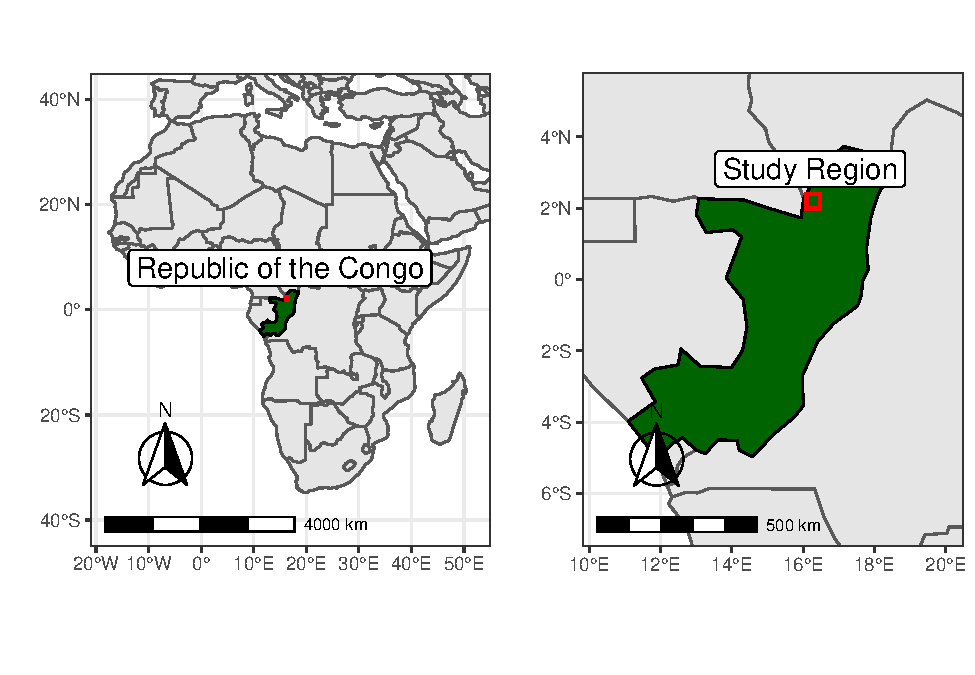
\includegraphics{Project_Template_files/figure-latex/mapping1-1.pdf}
\caption{Map displaying the location of the forest plots within the
Republic of Congo, Africa.}
\end{figure}

\begin{verbatim}
## Coordinate system already present. Adding new coordinate system, which will replace the existing one.
\end{verbatim}

\begin{figure}
\centering
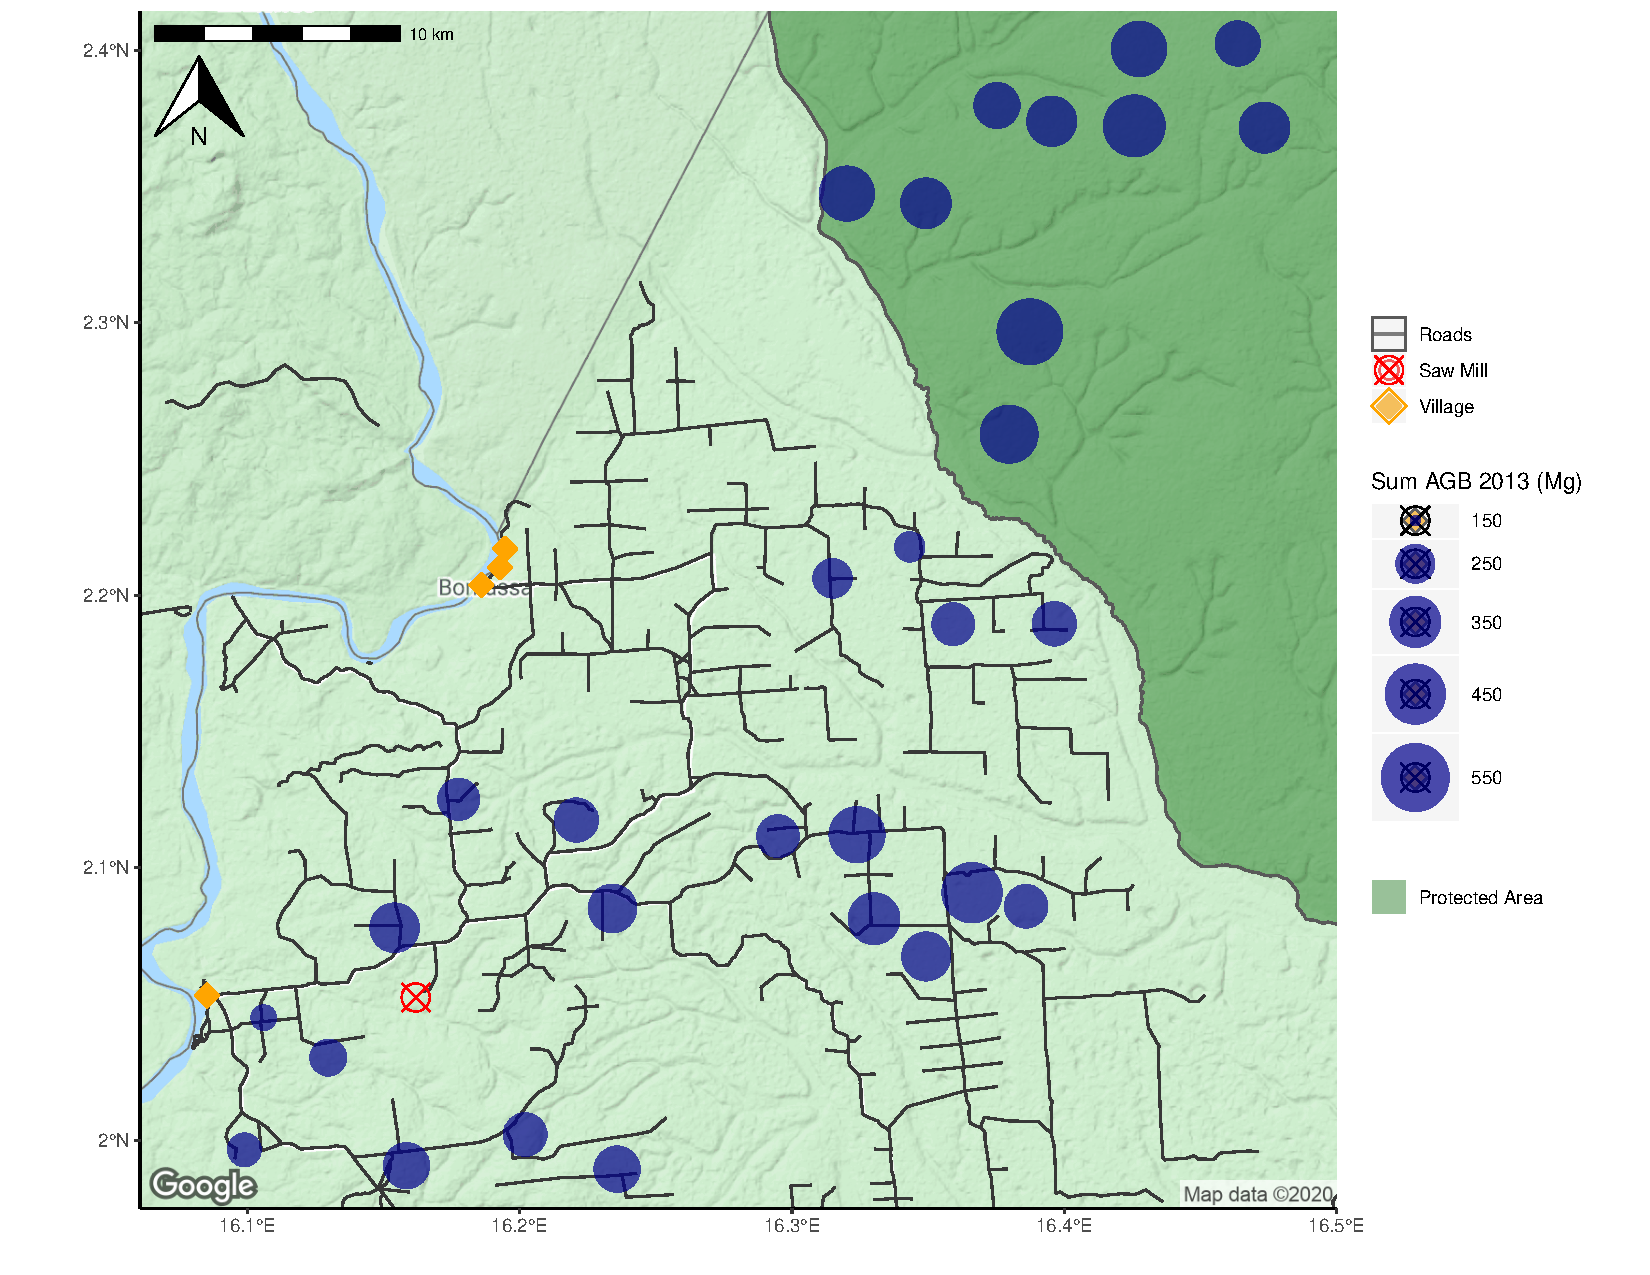
\includegraphics{Project_Template_files/figure-latex/mapping2-1.pdf}
\caption{Sum of above ground biomass (Mg) at each plot location in 2013.
Nearby road, village, saw mill, and protected area locations are plotted
to visualize the relationship between these variables and the amount of
above ground biomass.}
\end{figure}

\newpage

\hypertarget{summary-and-conclusions}{%
\section{Summary and Conclusions}\label{summary-and-conclusions}}

\newpage

\hypertarget{references}{%
\section{References}\label{references}}

Duncanson, L., Armston, J., Disney, M. et al.~The Importance of
Consistent Global Forest Aboveground Biomass Product Validation. Surv
Geophys 40, 979--999 (2019).
\url{https://doi.org/10.1007/s10712-019-09538-8} \textless{}add
references here if relevant, otherwise delete this section\textgreater{}


\end{document}
